\documentclass[12pt,letterpaper]{hmcpset}
\usepackage[margin=1in]{geometry}
\usepackage{graphicx}
\usepackage{amsmath}

% info for header block in upper right hand corner
\name{ }
\class{Math 60}
\assignment{HW 5}
\duedate{Monday, May 23, 2016}

\newcommand{\pn}[1]{\left( #1 \right)}
\newcommand{\abs}[1]{\left| #1 \right|}
\newcommand{\bk}[1]{\left[ #1 \right]}

\newcommand{\RR}{\mathbb{R}}

\renewcommand{\labelenumi}{{(\alph{enumi})}}

\begin{document}

\problemlist{3.3.24, 3.4.\{4, 7, 12, 13, 16, 23\}}

\begin{problem}[Colley 3.3.24]
    Consider the vector field
    $\textbf{F}=2x\textbf{i}+2y\textbf{j}-3\textbf{k}$.
    \begin{enumerate}
        \item Show that \textbf{F} is a gradient field.
        \item Describe the equipotential surfaces of \textbf{F} in
            words and with sketches.
    \end{enumerate}
\end{problem}
\begin{solution}
    \vfill
\end{solution}
\newpage

\begin{problem}[Colley 3.4.4]
    Calculate the divergence of the vector fields given in Exercises 1-6.
    \[
        \textbf{F}=z\cos(e^{y^2})\ \textbf{i}+x\sqrt{z^2+1}\ \textbf{j}
        +e^{2y}\sin3x\ \textbf{k}
    \]
\end{problem}
\begin{solution}
    \vfill
\end{solution}
\newpage

\begin{problem}[Colley 3.4.7]
    Find the curl of the vector fields given in Exercises 7-11.
    \[
        \textbf{F}=x^2\ \textbf{i}-xe^y\ \textbf{j}+2xyz\ \textbf{k}
    \]
\end{problem}
\begin{solution}
    \vfill
\end{solution}
\newpage

\begin{problem}[Colley 3.4.12]
    \begin{enumerate}
        \item Consider again the vector field in Exercise 8 and its
            curl. Sketch the vector field and use your picture to
            explain geometrically why the curl is as you calculated.
        \item Use geometry to determine $\nabla\times\textbf{F}$,
            where $\displaystyle\textbf{F}=\frac{(x\textbf{i}+y\textbf{j}
            +z\textbf{k})}{\sqrt{x^2+y^2+z^2}}$.
        \item For \textbf{F} as in part (b), verify your intuition by
            explicitly computing $\nabla\times\textbf{F}$.
    \end{enumerate}
\end{problem}
\begin{solution}
    \vfill
\end{solution}
\newpage

\begin{problem}[Colley 3.4.13]
    Can you tell in what portions of $\RR^2$, the vector fields shown
    in Figures 3.43-3.46 have positive divergence? Negative
    divergence?
    \begin{center}
        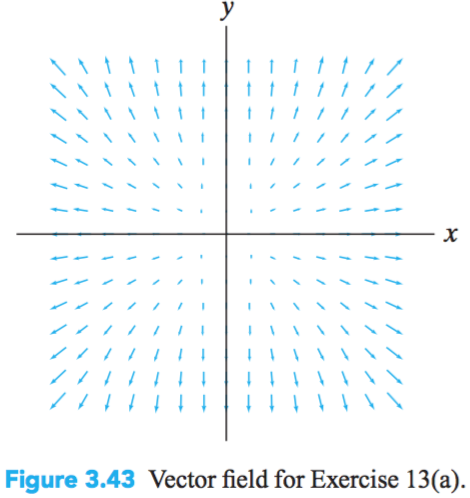
\includegraphics[scale=0.8]{img/3_4_13a}\qquad
        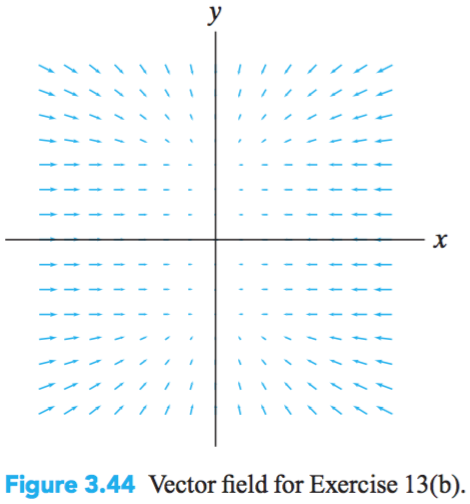
\includegraphics[scale=0.8]{img/3_4_13b}\\
        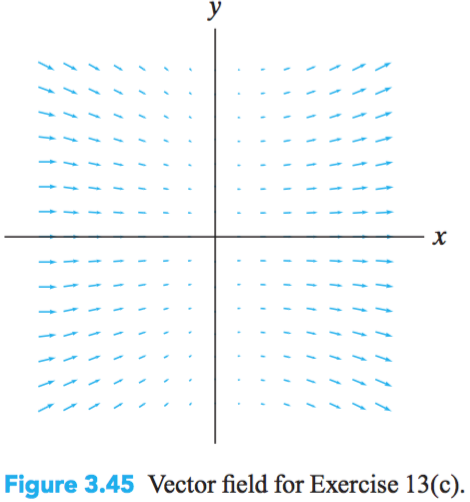
\includegraphics[scale=0.8]{img/3_4_13c}\qquad
        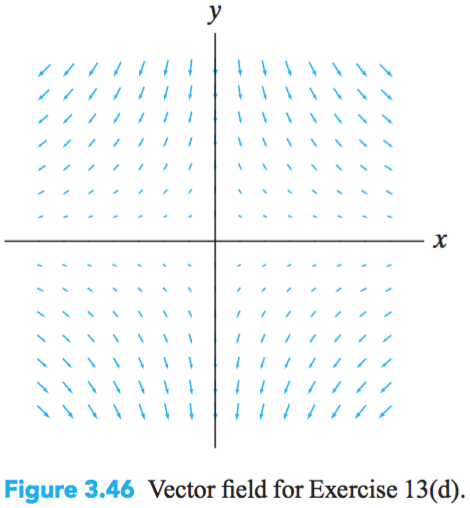
\includegraphics[scale=0.8]{img/3_4_13d}
    \end{center}
\end{problem}
\begin{solution}
    \vfill
\end{solution}
\newpage

\begin{problem}[Colley 3.4.16]
    Prove Theorem 4.4.
\end{problem}
\begin{solution}
    \vfill
\end{solution}
\newpage

\begin{problem}[Colley 3.4.23]
    In Exercises 21-25, establish the given identities. (You may
    assume that any functions and vector fields are appropriately
    differentiable.)
    \[
        \nabla\cdot(f\textbf{F})=f\nabla\cdot\textbf{F}+\textbf{F}\cdot\nabla f
    \]
\end{problem}
\begin{solution}
    \vfill
\end{solution}
\end{document}
